\section{Physarum Polycephalum}
\label{section:background_physarum}

The organism being a subject for this work is \textit{Physarum Polycephalum} also called the many-headed slime mould. It is a member of the \textit{Physaridae} family of slime moulds, in order of \textit{Physarales}, class \textit{Myxogastria}, phylum \textit{Myxomycete}, supergroup \textit{Amoebozoa} in \textit{Protista} kingdom. While current position in taxology is well defined, presented characteristics will justify why scientists used to have problems with classification of the Physarum \cite{stephenson1994myxomycetes}.

In order to make the thesis readable, terms \textit{Physarum Polycephalum}, \textit{Physarum} or \textit{the slime mould} will be used interchangeably as the subject is unambiguously defined. As none of the authors have a background in biology, concepts are presented from a computer scientist's perspective in minimal, yet exhaustive, form.


\subsection{Biological characteristics}

\textit{Physarum Polycephalum} is a very peculiar organism. Even being a \textit{Protista} it can be observed with a naked eye --- it is a one amongst biggest living unicellular ogranisms \cite{TODO}. 

In its natural habitat, under cool, dark and humid conditions the slime mould exists in form of a yellow semistructurized blob (as seen in figure \ref{figure:bp_habitat}). Its occurrence is fairly common around the globe, however species \textit{Physarum Polycephalum} does not occur naturally in Poland \cite{narkiewicz2013grzyby}. It feeds on bacteria, fungi and other sources of basic nutrients.

In labaratory conditions, \textit{Physarum} is stored on Petri dishes filled with non-nutritious agar (figure \ref{figure:bp_petri}). The agar base provides humid environment required for supporting plasmodial stage of the slime mould. A sterille oats or even soft porridge is used as controlled source of nutrients. Complete description of storage and observation protocol, among other informations, is provided in Appendix \ref{chapter:protocol}.

\begin{figure}
  \centering
  % TODO find another image
  \begin{subfigure}{0.45\textwidth}
    \centering
    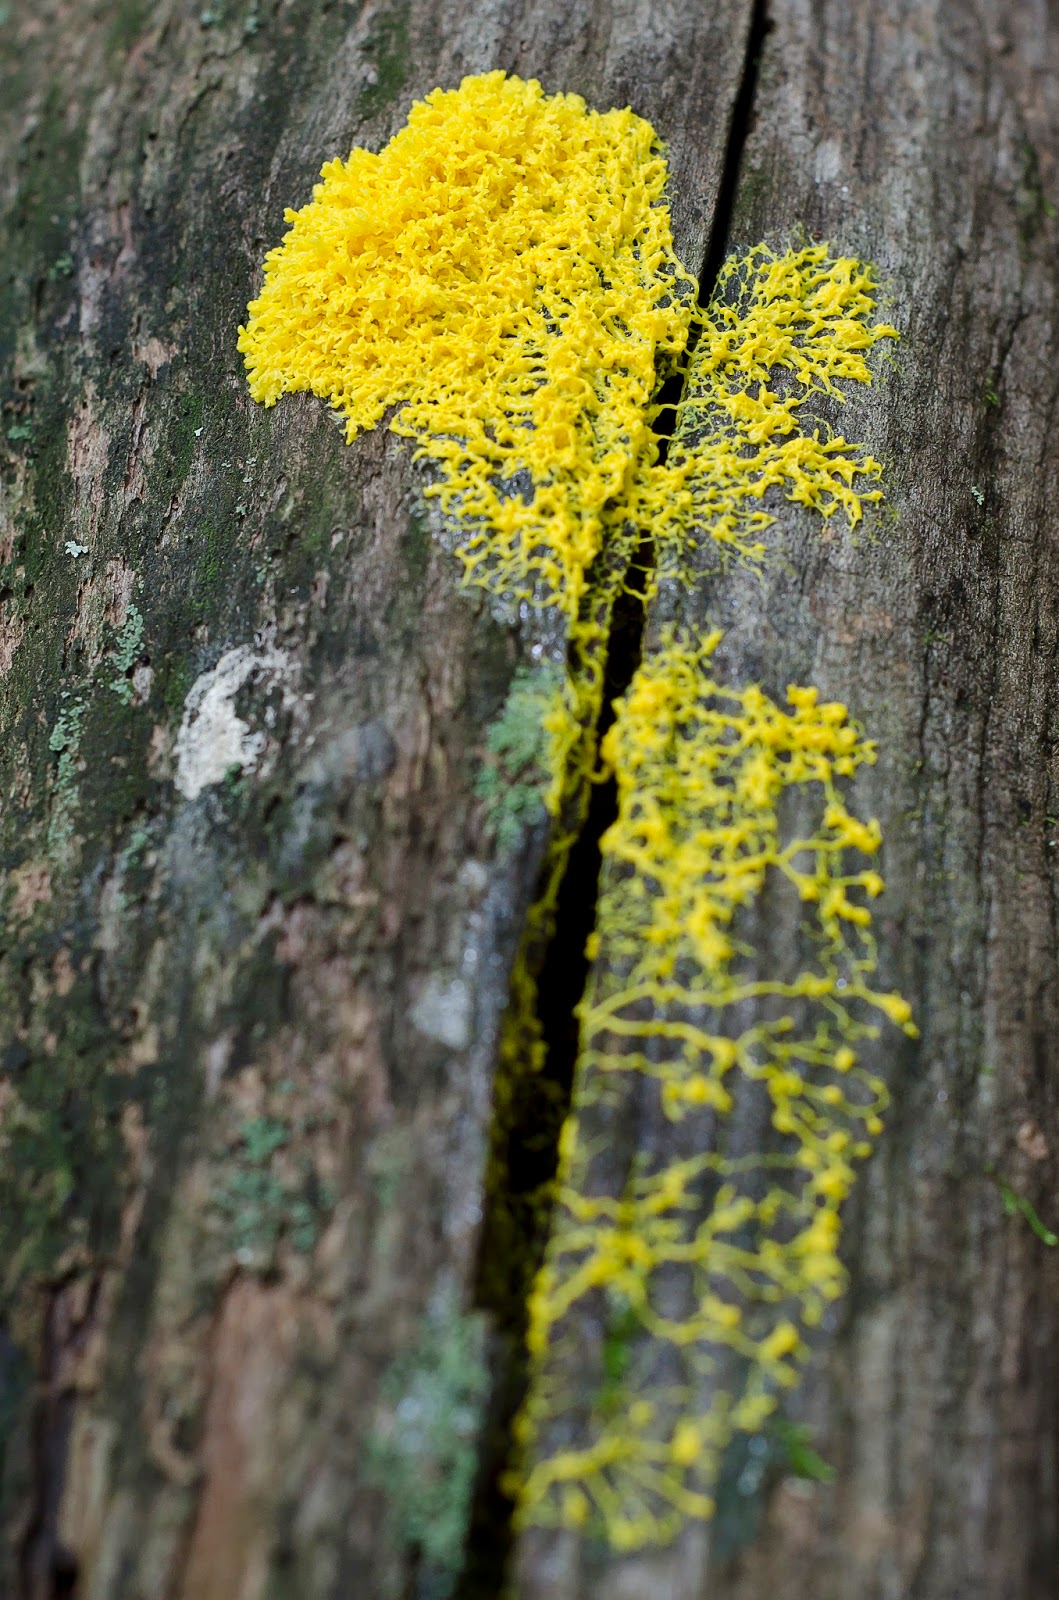
\includegraphics[width=0.44\textwidth]{background/physarum/habitat.jpg}
    \caption{Natural habitat \cite{TODO}}
    \label{figure:bp_habitat}
  \end{subfigure}
  \begin{subfigure}{0.45\textwidth}
    \centering
    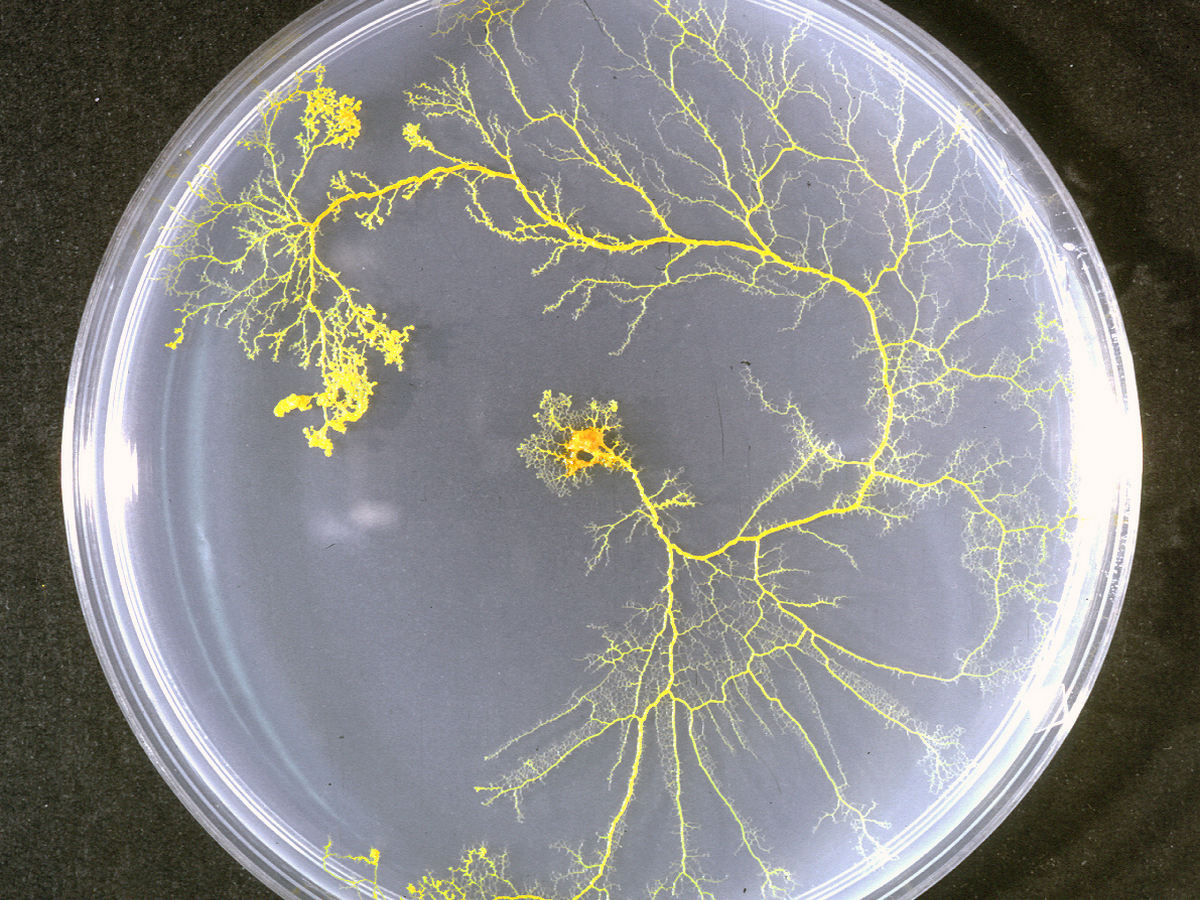
\includegraphics[width=0.9\textwidth]{background/physarum/petri.jpg}
    \caption{Petri dish}
    \label{figure:bp_petri}
  \end{subfigure}
  \caption{\textit{Physarum Polycephalum} in plasodial stage}
\end{figure}

% TODO preferred image from carolina
\begin{figure}
  \centering
  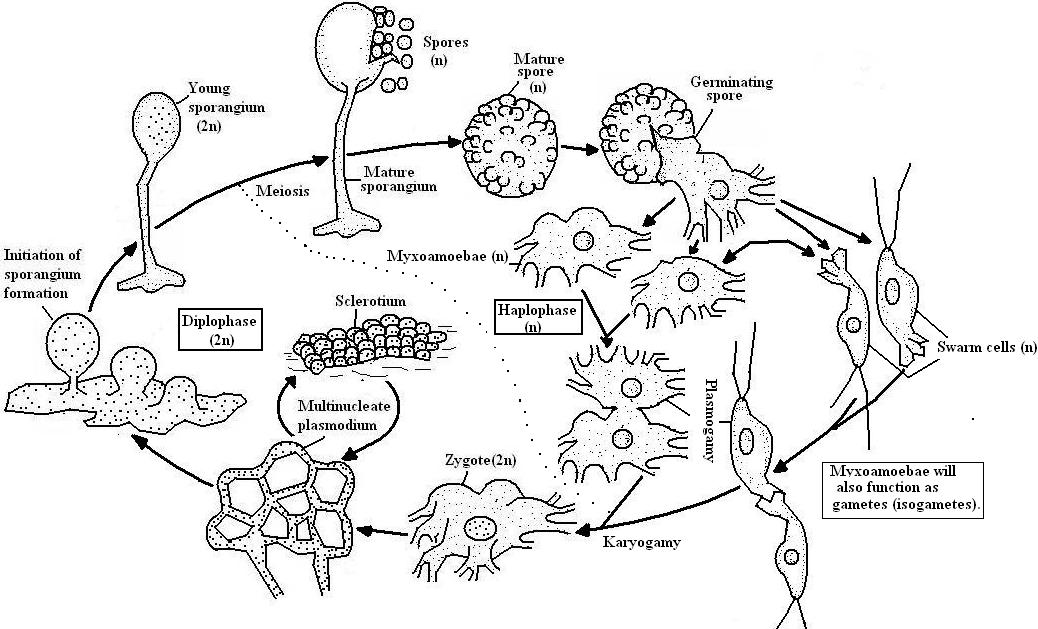
\includegraphics[width=0.94\textwidth]{background/physarum/lifecycle.png}
  \caption{Lifecycle of \textit{Physarum Polycephalum} \cite{TODO}}
  \label{figure:bp_lifecycle}
\end{figure}

As representant of \textit{Myxomycete}, a life cycle of the slime mould is very complex including haploid and diploid phases (as seen in figure \ref{figure:bp_lifecycle}). Such cycle is result of evolutionary adaptation. Formation of sporangium occurs in result of worsening conditions (such as inadequate temperature, humidity or acidity). Sporangium releases spores, which can germinate into ameboid swarm cell. Such cell can enclose itself into a cyst to protect the cells until environmental conditions improve. When conditions are favourable amoeboid cell turns into flagellated swarm cell. Swarm cells can merge, fuse their nuclei and start mitotic process resulting in forming a plasmodium \cite{jones2015pattern}.

For purposes of unconventional computing applications, \textit{Physarum} is preferred in its such plasmodial stage. However, during research transformations into other states are inevitable and must be dealt with. In case of drying and enforced starvation sclerotium is formed --- in this dormant phase \textit{Physarum Polycephalum} can survive for many years until dampness and nutrients are provided again.

Plasmodium forms protoplasmic tubes (also called pseudopodia) accordingly to food availability. Such tubes are used for discovery and transportation of nutrients. The tubes are built in similar way to animal muscles. The ectoplasm contains actin and myosin complexes, which are organised into regular structures forming tubes. Such actomyosin complexes generate contractile motion resulting in streaming of protoplasm. Furthermore, synchronized oscillations of protoplasm stream direction can observed. Nutrients are transported in one direction, after 1-2~minutes the direction is reversed. Period of this oscillation depends on environment quality and accesibility to food \cite{wohlfarth1979oscillatory} --- higher frequency oscillations are generated where nutrients available and no harmful environment exist, low frequency oscillations are caused by lack of food or as a result of unfavourable conditions. 

The plasmodium can grow around 10~mm per hour when actively exploring environment \cite{coggin1996dynamic}. While moving, plasmodium leaves polysaccharide traces (informally called slime, hence the name slime mould). Network of the protoplasmic tubes adapts, forming efficient ways of transporting nutrients, depending on their amount and quality \cite{nakagaki2004obtaining}. Usage of this behaviour is a fundamental principle for building physarum machines.


\subsection{Related works}

Since early 1960s \textit{Physarum Polycephalum} has been a subject to many biological and microbiological studies \cite{guttes1964mitotic,daniel1962method}, however it is late 70s when its computational-like behaviours have been observed \cite{wohlfarth1979oscillatory}.

% TODO ref names places
Research towards computational applications of the \textit{Physarum} truly started in 1990s. Nowadays, there exist two prominent research centers focusing on the slime mould --- one based in United Kingdom, other one in Japan. Some of their works excited us about slime mould capabilities and inspired to write this thesis.  Presented here experiments with their results focus on different aspects of \textit{Physarums} behaviour. Analyzing and understanding them gives impression of emerging computational power of such simple organism as a slime mould.


\subsubsection{Maze-solving capabilities}

% TODO ref
Maze-solving or more constricted problem of finding, preferably shortest, paths is a very common in practice. It has many applications and many possible algorithms are already available. Algorithms such as breadth-first search or more complex $A*$ are commonly used for solving mazes, however Toshiyuki Nakagaki et al. proposed usage slime moulds' natural capabilities as unconventional solution to this problem.

% TODO wrzucic obrazek
In order to use \textit{Physarum} to solve a labiryth, a maze must be represented as a physical object. Such maze is modelled on a Petri dish where floor is made of non-nutrient agar and walls are made of thin plastic film (the maze used in the experiment is presented on figure \ref{figure:bp_maze}). As the slime mould strictly prefers humid environment of the agar it will not pass arid walls made of plastic film. 

There are four possible routes available $\{(\alpha_1,\beta_1), (\alpha_1,\beta_2), (\alpha_2,\beta_1), (\alpha_2,\beta_2)\}$ between entry point $A$ and exit point $B$. Oatmeal-agar based source of nutrients is planted in both entry and exit points, while large enough plasmodium is placed over whole floor of the maze. As time passes it can be observed that plasmodium retracts its body from labirth's dead-ends, leaving traces of slime where it previously has been placed. 

As a result the slime mould rests only on direct paths connecting an entry with an exit point. Furthermore, it has been observed that \textit{Physarum Polycephalum} usually prefers shortest $(\alpha_2,\beta_1)$ path as it prefers most efficient way for transferring nutrients. 


\subsubsection{Spatial memory}

lorem y-shaped


\subsubsection{Adaptive network design}

lorem tokyo


\subsection{Observations}

lorem


\subsubsection{Sensoric input}

% nasa gravisens
lorem


\subsection{Computer models}

lorem


